\documentclass[journal,12pt,twocolumn]{IEEEtran}
\usepackage{setspace}
\usepackage{gensymb}
\usepackage{xcolor}
\usepackage{caption}
\singlespacing
\usepackage{siunitx}
\usepackage[cmex10]{amsmath}
\usepackage{mathtools}
\usepackage{hyperref}
\usepackage{amsthm}
\usepackage{mathrsfs}
\usepackage{txfonts}
\usepackage{stfloats}
\usepackage{cite}
\usepackage{cases}
\usepackage{subfig}
\usepackage{longtable}
\usepackage{multirow}
\usepackage{enumitem}
\usepackage{bm}
\usepackage{mathtools}
\usepackage{listings}
\usepackage{tikz}
\usetikzlibrary{shapes,arrows,positioning}
\usepackage{circuitikz}
\renewcommand{\vec}[1]{\boldsymbol{\mathbf{#1}}}
\DeclareMathOperator*{\Res}{Res}
\renewcommand\thesection{\arabic{section}}
\renewcommand\thesubsection{\thesection.\arabic{subsection}}
\renewcommand\thesubsubsection{\thesubsection.\arabic{subsubsection}}

\renewcommand\thesectiondis{\arabic{section}}
\renewcommand\thesubsectiondis{\thesectiondis.\arabic{subsection}}
\renewcommand\thesubsubsectiondis{\thesubsectiondis.\arabic{subsubsection}}
\hyphenation{op-tical net-works semi-conduc-tor}

\lstset{
language=Python,
frame=single, 
breaklines=true,
columns=fullflexible
}
\begin{document}
\theoremstyle{definition}
\newtheorem{theorem}{Theorem}[section]
\newtheorem{problem}{Problem}
\newtheorem{proposition}{Proposition}[section]
\newtheorem{lemma}{Lemma}[section]
\newtheorem{corollary}[theorem]{Corollary}
\newtheorem{example}{Example}[section]
\newtheorem{definition}{Definition}[section]
\newcommand{\BEQA}{\begin{eqnarray}}
\newcommand{\EEQA}{\end{eqnarray}}
\newcommand{\define}{\stackrel{\triangle}{=}}
\newcommand{\myvec}[1]{\ensuremath{\begin{pmatrix}#1\end{pmatrix}}}
\newcommand{\mydet}[1]{\ensuremath{\begin{vmatrix}#1\end{vmatrix}}}
\bibliographystyle{IEEEtran}
\providecommand{\nCr}[2]{\,^{#1}C_{#2}} % nCr
\providecommand{\nPr}[2]{\,^{#1}P_{#2}} % nPr
\providecommand{\mbf}{\mathbf}
\providecommand{\pr}[1]{\ensuremath{\Pr\left(#1\right)}}
\providecommand{\qfunc}[1]{\ensuremath{Q\left(#1\right)}}
\providecommand{\sbrak}[1]{\ensuremath{{}\left[#1\right]}}
\providecommand{\lsbrak}[1]{\ensuremath{{}\left[#1\right.}}
\providecommand{\rsbrak}[1]{\ensuremath{{}\left.#1\right]}}
\providecommand{\brak}[1]{\ensuremath{\left(#1\right)}}
\providecommand{\lbrak}[1]{\ensuremath{\left(#1\right.}}
\providecommand{\rbrak}[1]{\ensuremath{\left.#1\right)}}
\providecommand{\cbrak}[1]{\ensuremath{\left\{#1\right\}}}
\providecommand{\lcbrak}[1]{\ensuremath{\left\{#1\right.}}
\providecommand{\rcbrak}[1]{\ensuremath{\left.#1\right\}}}
\theoremstyle{remark}
\newtheorem{rem}{Remark}
\newcommand{\sgn}{\mathop{\mathrm{sgn}}}
\newcommand{\rect}{\mathop{\mathrm{rect}}}
\newcommand{\sinc}{\mathop{\mathrm{sinc}}}
\providecommand{\abs}[1]{\left\vert#1\right\vert}
\providecommand{\res}[1]{\Res\displaylimits_{#1}} 
\providecommand{\norm}[1]{\lVert#1\rVert}
\providecommand{\mtx}[1]{\mathbf{#1}}
\providecommand{\mean}[1]{E\left[ #1 \right]}
\providecommand{\fourier}{\overset{\mathcal{F}}{ \rightleftharpoons}}
\providecommand{\ztrans}{\overset{\mathcal{Z}}{ \rightleftharpoons}}
\providecommand{\system}[1]{\overset{\mathcal{#1}}{ \longleftrightarrow}}
\newcommand{\solution}{\noindent \textbf{Solution: }}
\providecommand{\dec}[2]{\ensuremath{\overset{#1}{\underset{#2}{\gtrless}}}}
\let\StandardTheFigure\thefigure
\def\putbox#1#2#3{\makebox[0in][l]{\makebox[#1][l]{}\raisebox{\baselineskip}[0in][0in]{\raisebox{#2}[0in][0in]{#3}}}}
     \def\rightbox#1{\makebox[0in][r]{#1}}
     \def\centbox#1{\makebox[0in]{#1}}
     \def\topbox#1{\raisebox{-\baselineskip}[0in][0in]{#1}}
     \def\midbox#1{\raisebox{-0.5\baselineskip}[0in][0in]{#1}}

\vspace{3cm}
\title{Line Assignment}
\author{Gautam Singh}
\maketitle
\bigskip

\begin{abstract}
    This document contains the solution to Question 16 of Exercise 2 in Chapter
    11 of the class 12 NCERT textbook.
\end{abstract}

\begin{enumerate}
    \item Find the shortest distance between the lines whose vector equations are
    \begin{align}
        \vec{x} = \myvec{1\\2\\3} + \lambda_1\myvec{1\\-3\\2}
        \label{eq:L1}
    \end{align}
    and
    \begin{align}
        \vec{x} = \myvec{4\\5\\6} + \lambda_2\myvec{2\\3\\1}
        \label{eq:L2}
    \end{align}

    \solution Suppose there are two lines in general given by
    \begin{align}
        \vec{x} = \vec{x_1} + \lambda_1\vec{m_1} \label{eq:L1-gen} \\
        \vec{x} = \vec{x_2} + \lambda_2\vec{m_2} \label{eq:L2-gen}
    \end{align}
    If these lines intersect, then
    \begin{align}
        \lambda_1\vec{m_1} - \lambda_2\vec{m_2} &= \vec{x_2} - \vec{x_1} \\
        \implies \vec{M}\vec{\lambda} &= \vec{x_2} - \vec{x_1}
        \label{eq:intersect-cond}
    \end{align}
    where
    \begin{align}
        \vec{M} \triangleq \myvec{\vec{m_1} & \vec{m_2}} \label{eq:M-def} \\
        \vec{\lambda} \triangleq \myvec{\lambda_1\\-\lambda_2}
        \label{eq:lambda-def}
    \end{align}
    In this case,
    \begin{align}
        \vec{x_1} = \myvec{1\\2\\3} \quad \vec{x_2} = \myvec{4\\5\\6}
        \quad \vec{m_1} = \myvec{1\\-3\\2} \quad \vec{m_2} = \myvec{2\\3\\1}
        \label{eq:vals}
    \end{align}
    To check whether \eqref{eq:intersect-cond} has a solution in $\vec{\lambda}$,
    we use the augmented matrix.
    \begin{align}
        \myvec{1&2&3\\-3&3&3\\2&1&3} &\xleftrightarrow[]{R_2\leftarrow R_2+3R_1} \myvec{1&2&3\\0&9&12\\2&1&3} \\
                &\xleftrightarrow[]{R_3\leftarrow R_3-2R_1} \myvec{1&2&3\\0&9&12\\0&-3&-3} \\
                &\xleftrightarrow[]{R_3\leftarrow 3R_3+R_2} \myvec{1&2&3\\0&9&12\\0&0&3}
                \label{eq:rank-aug}
    \end{align}
    Clearly, the rank of this matrix is 3, and therefore, the lines are skew.

    Now, suppose that the closest points on both lines are
    \begin{align}
        \vec{A} = \vec{x_1} + \lambda_1\vec{m_1} \label{eq:a-def} \\
        \vec{B} = \vec{x_2} + \lambda_2\vec{m_2}
        \label{eq:b-def}
    \end{align}
    Then, $AB$ is perpendicular to both lines, hence
    \begin{align}
        \vec{m_1}^\top\brak{\vec{A}-\vec{B}} = 0 \\
        \vec{m_2}^\top\brak{\vec{A}-\vec{B}} = 0 \\
        \implies \vec{M}^\top\brak{\vec{A}-\vec{B}} = \vec{0}
        \label{eq:perp-vec}
    \end{align}
    Using \eqref{eq:a-def} and \eqref{eq:b-def} in \eqref{eq:perp-vec},
    \begin{align}
        \vec{M}^\top\brak{\vec{x_1}-\vec{x_2} + \vec{M}\vec{\lambda}} = \vec{0} \\
        \implies \vec{M^\top M\lambda} = \vec{M}^\top\brak{\vec{x_2}-\vec{x_1}}
        \label{eq:lambda-eqn}
    \end{align}
    Substituting from \eqref{eq:vals} in \eqref{eq:lambda-eqn} and forming the 
    augmented matrix,
    \begin{align}
        \myvec{14&-5&0\\-5&14&18} &\xleftrightarrow[]{R_1\leftarrow R_1+R_2} \myvec{9&9&18\\-5&14&18} \\
                 &\xleftrightarrow[]{R_1\leftarrow\frac{R_1}{9}} \myvec{1&1&2\\-5&14&18} \\
                 &\xleftrightarrow[]{R_2\leftarrow R_2+5R_1} \myvec{1&1&2\\0&19&28} \\
                 &\xleftrightarrow[]{R_1\leftarrow19R_1-R_2} \myvec{19&0&10\\0&19&28} \\
                 &\xleftrightarrow[]{\substack{R_1\leftarrow\frac{R_1}{19}\\R_2\leftarrow\frac{R_2}{9}}}
                    \myvec{1&0&\frac{10}{19}\\0&1&\frac{28}{19}} \\
                    \implies \vec{\lambda} &= \frac{1}{19}\myvec{10\\28}
        \label{eq:lambda-sol}
    \end{align}
    Hence, using \eqref{eq:lambda-def} and substituing into \eqref{eq:a-def} and \eqref{eq:b-def},
    \begin{align}
        \vec{A_m} = \frac{1}{19}\myvec{29\\8\\77},\ \vec{B_m} = \frac{1}{19}\myvec{20\\11\\86}
    \end{align}
    Thus, the required distance is
    \begin{align}
        \norm{\vec{B_m}-\vec{A_m}} = \frac{\sqrt{9^2 +3^2 +(-9)^2}}{19} = \frac{3}{\sqrt{19}}
    \end{align}
    The situation is depicted in Fig. \ref{fig:skew}.

    \begin{figure}[!ht]
        \centering
        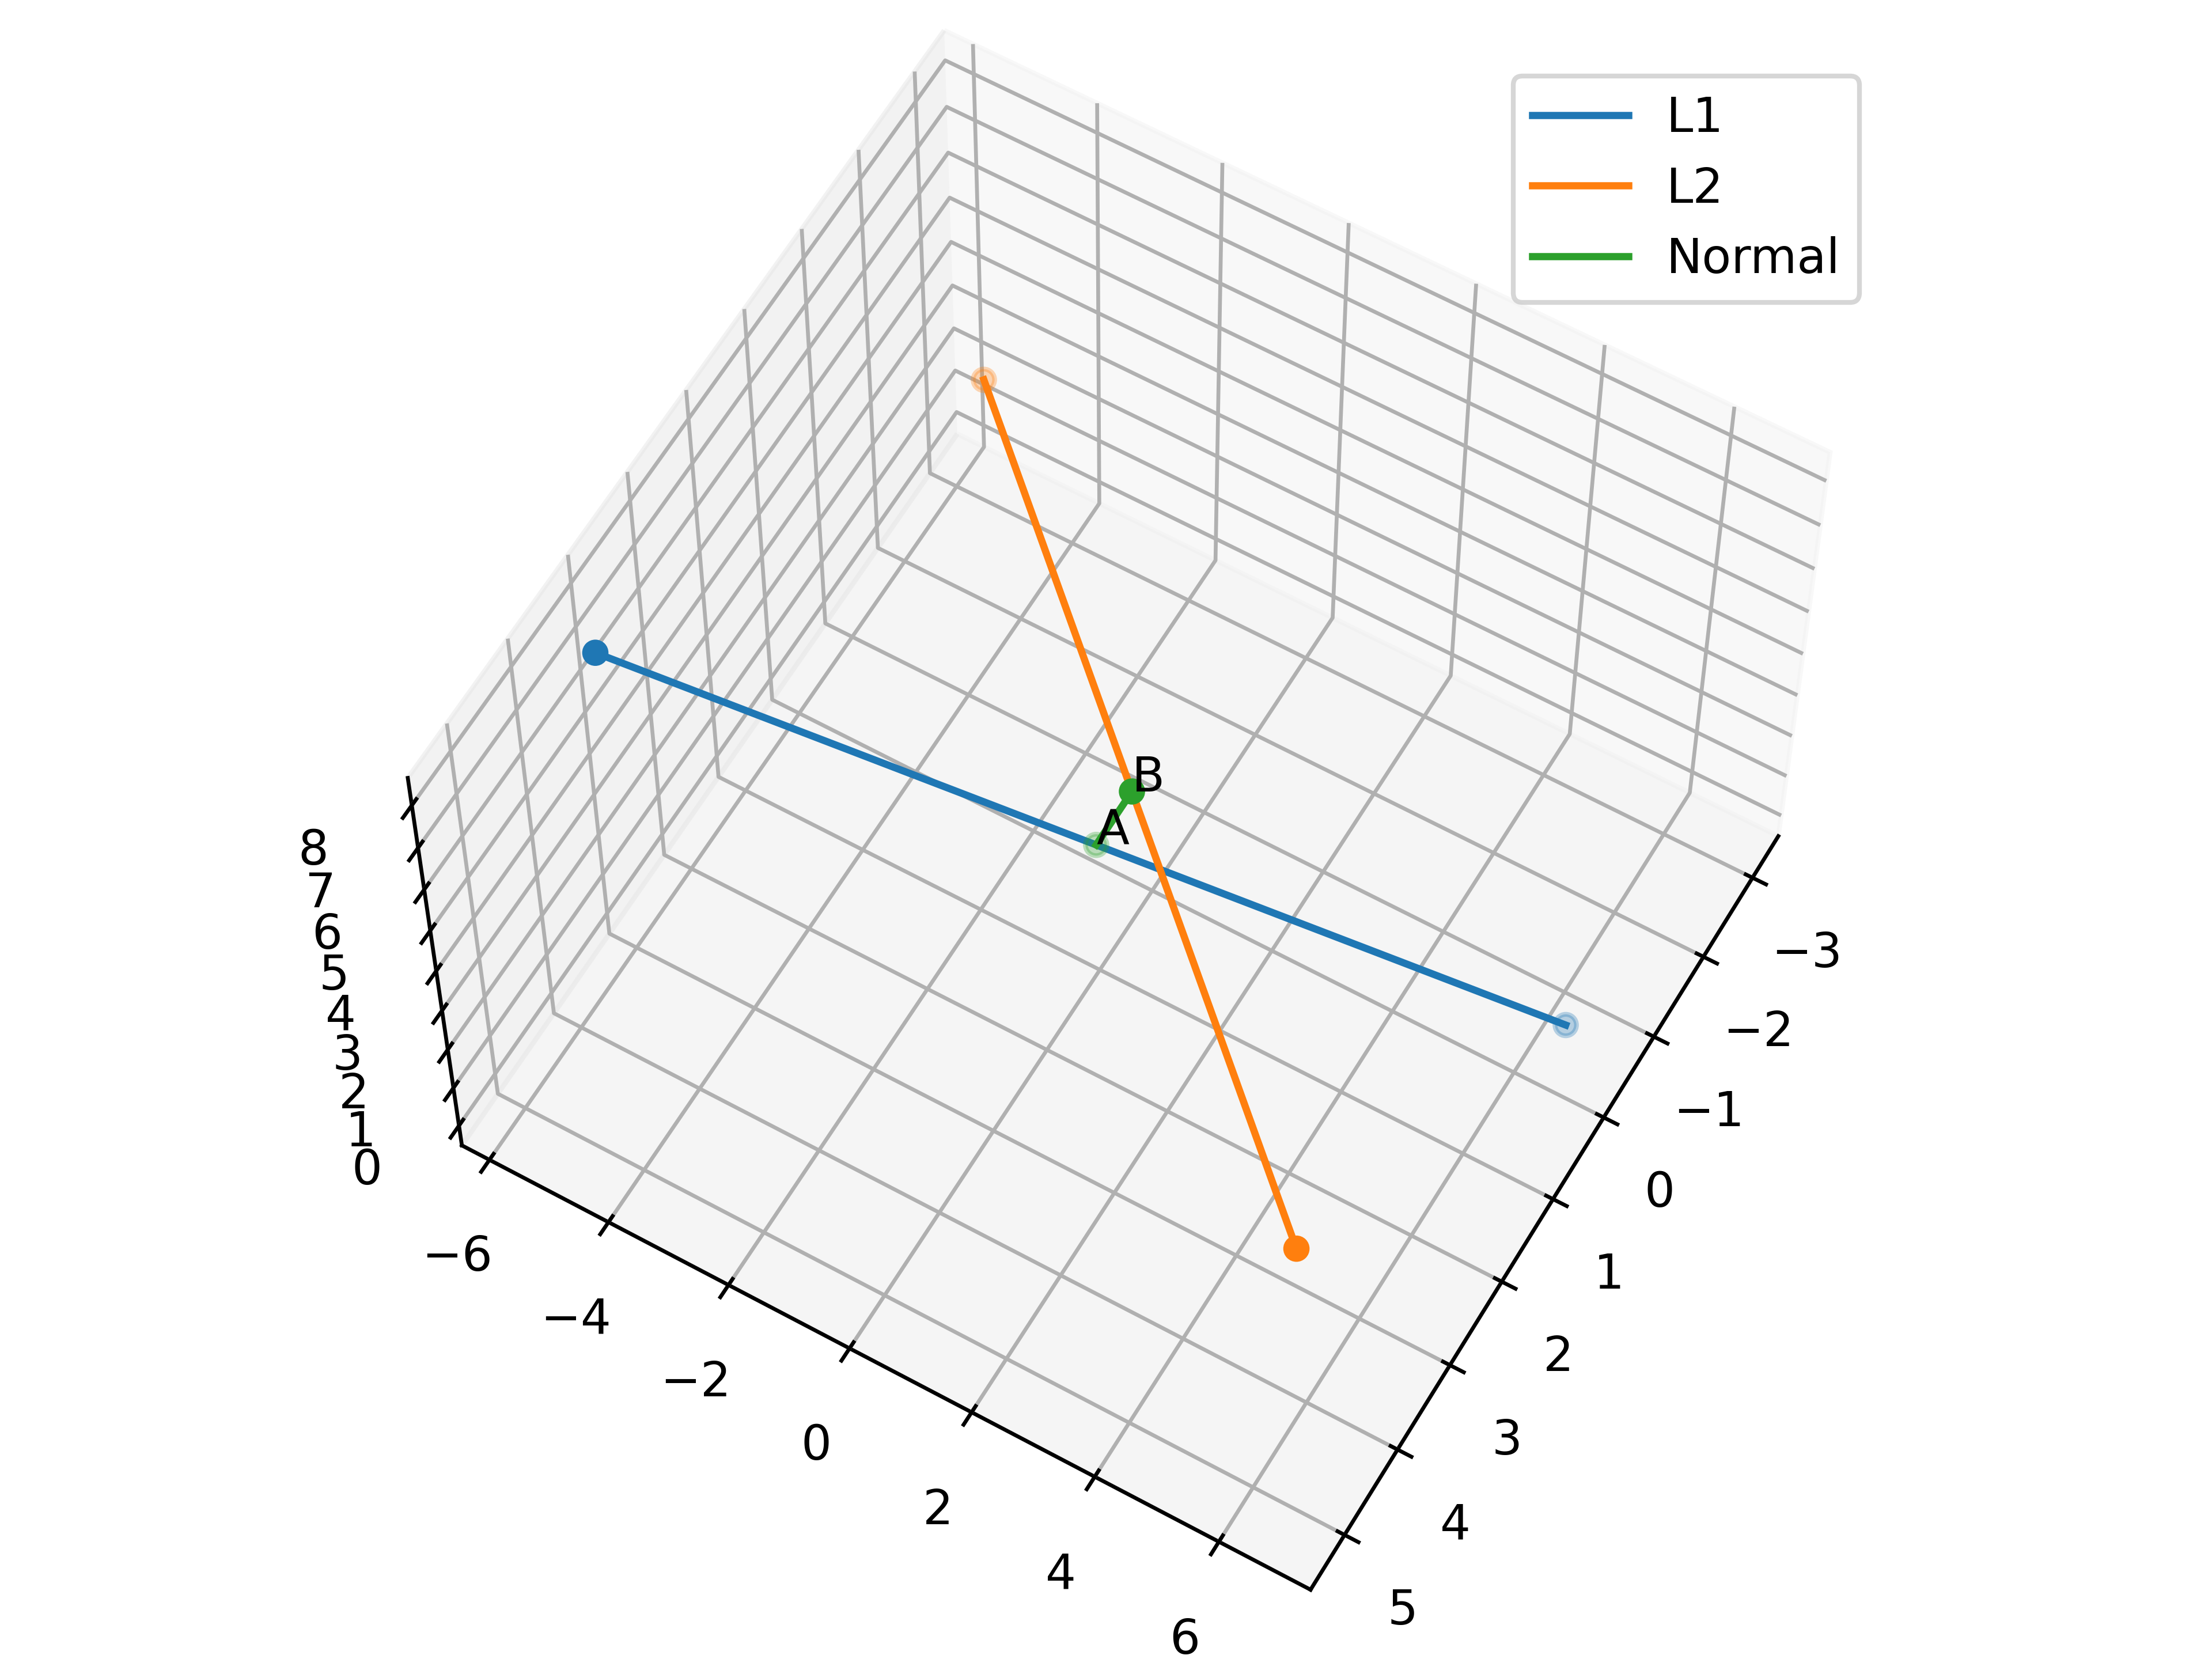
\includegraphics[width=\columnwidth]{figs/skew.png}
        \caption{$AB$ is the required shortest distance.}
        \label{fig:skew}
    \end{figure}
\end{enumerate}
\end{document}
